\section{Lecture 7, McCulloch Pitts Neuron and Perceptron Learning Algorithm}
\subsection{McCulloch-Pitts Neuron}
\begin{tabular}{p{4cm}p{15cm}}
 States of a neuron	& Only two states: Active (1) or inactive (0)\\
 Electric symbol	& 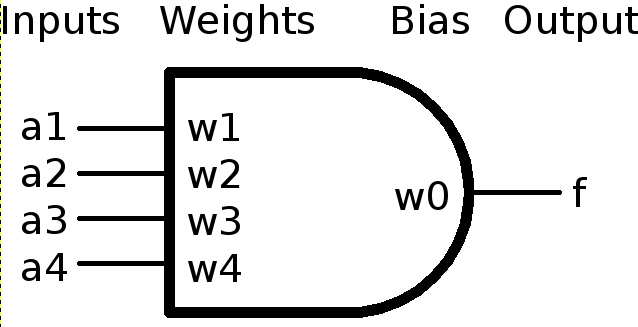
\includegraphics[width = 10cm]{neuroinf_mccullochpitts.png}\\
			& \begin{tabular}[t]{llp{10cm}}
			  Inputs	& bool*		& Input vector represents dendrites. If a presynaptic cell activates a dendrite, the respective vector element is 1.\\
			  Weights	& float*	& Represents efficiency of a synapse. $w < 0$ represents inhibitory signals, $w > 0$ represents excitatory signals.\\
			  Bias		& float		& \\
			  Output	& bool		& $f = \left( \sum_i a_i w_i + w_0 \geq 0 \right)$. The sum represents the soma, which integrates all potentials from the dendrites. $f$ represents whether the neuron spikes or not.
			  \end{tabular}\\
 Examples		& \begin{tabular}[t]{lll}
			    $w = \{1,1\}$	& $-2 < w_o < -1$	& AND-Gate\\
			    $w = \{1,1\}$	& $-1 < w_o \leq -1$	& OR-Gate\\
			    $w = \{-1\}$	& $w = 0$		& NOT-Gate
			  \end{tabular}\\
XOR-Problem		& The XOR-Gate can't be modeled by a single McCulloch Pitts Neuron.\\
Proof			& \begin{tabular}[t]{p{15cm}}
			    Let $(a_1,a_2)$ be the input vector, $(w_1,w_2)$ the corresponding weight vector, $w_0$ the bias and $f$ the output boolean.\\
			    The equation modeling the MCP-Neuron is then $a_1w_1 + a_2w_2 + w_O \geq 0 = f$\\
			    The truth table for the XOR-Gate reads as follows\\
			    \begin{tabular}{|cc|c|}
			    \toprule
			    $a_1$	& $a_2$	& $f$\\\midrule
			    0		& 0	& 0\\
			    1		& 0	& 1\\
			    0		& 1	& 1\\
			    1		& 1	& 0\\\bottomrule
			    \end{tabular}\\
			    The following system of inequalities arises from that truth table\\
			    \begin{tabular}{ccccccc}
			            &   &       &   & $w_0$ & $<$    & 0\\    
			            &   & $w_2$ & + & $w_0$ & $\geq$ & 0\\    
			      $w_1$ &   &       & + & $w_0$ & $\geq$ & 0\\    
			      $w_1$ & + & $w_2$ & + & $w_0$ & $<$    & 0\\
			     \end{tabular}\\
			     By linear combination, one finds that $w_1 + w_2 + 2w_0 \geq 0$ AND $w_1 + w_2 + 2w_0 < 0$ must hold, which is a contradiction.
			   \end{tabular}
\end{tabular}
\subsection{Perceptron learning algorithm}
Folgende �berlegungen liegen der Lernregel des Perzeptrons zu Grunde:
\begin{enumerate}
 \item Wenn die Ausgabe eines Neurons 1 (bzw. 0) ist und den Wert 1 (bzw. 0) annehmen soll, dann werden die Gewichtungen nicht ge�ndert.
 \item Ist die Ausgabe 0, soll aber den Wert 1 annehmen, dann werden die Gewichte inkrementiert.
 \item Ist die Ausgabe 1, soll aber den Wert 0 annehmen, dann werden die Gewichte dekrementiert.
\end{enumerate}
Mathematisch wird der Sachverhalt folgendermassen ausgedr�ckt:\\
Sei $\vec{x}$ der Eingabevektor, $\vec{w}$ der Gewichtsvektor und $0 < \alpha < 1$ der Lerngeschwindigkeits-Koeffizient\\
Eine Gewichtsaktualisierung im Schritt $k$ verl�uft wie folgt:
\begin{enumerate}
 \item $w(k+1) = w(k)$ bei korrekter Ausgabe,
 \item $w_j(k+1) = w_j(k) + \alpha x_{j}$ bei Ausgabe 0 und gew�nschter Ausgabe 1 und
 \item $w_j(k+1) = w_j(k) - \alpha x_{j}$ bei Ausgabe 1 und gew�nschter Ausgabe 0.
\end{enumerate}